% \documentclass[10pt,journal,cspaper,compsoc]{IEEEtran}
\documentclass[10pt,twocolumn,letterpaper]{article}
\usepackage{cvpr}
\usepackage{times}
\usepackage{graphicx}
\usepackage[pagebackref=true,breaklinks=true,letterpaper=true,colorlinks,bookmarks=false]{hyperref}

\cvprfinalcopy % *** Uncomment this line for the final submission

\def\cvprPaperID{****} % *** Enter the CVPR Paper ID here
\def\httilde{\mbox{\tt\raisebox{-.5ex}{\symbol{126}}}}

% Pages are numbered in submission mode, and unnumbered in camera-ready
\ifcvprfinal\pagestyle{empty}\fi
\begin{document}

%%%%%%%%% TITLE
\title{Using Bayesian Learning to Estimate How Hot an Execution Path is}

\author{Karim Ali\\
David R. Cheriton School of Computer Science\\
University of Waterloo\\
{\tt\small karim@uwaterloo.ca}}

\maketitle
\thispagestyle{empty}

\begin{abstract}
   
\end{abstract}

% \section{Problem Domain}

% 
% \section{Existing Solutions}
% Static profiling has been commonly used in the literature to identify hot paths. Although static profiling can be very useful and successful, it faces many
% practical challenges:
% \begin{enumerate}
%   \item the frequent lack of appropriate workloads for programs,
%   \item the questionable degree to which they are indicative of actual usage,
%   \item the inability of such tools evaluate program modules or individual paths in isolation,
%   \item and the extra work done by the programmer/developer to write code that generates program profiles.
% \end{enumerate}
% 
% Analyzing additional information, e.g data flow analysis \cite{boogerd2008use},  is also a common practice that helps identify hot paths.
% 
% \section{Interesting Solution}
% Raymond Buse and Westley Weimer \cite{buse2009road} propose a very interesting approach to the problem of hot paths identification. The proposed solution is
% modelled as a classification problem, where a path is classified as \textsf{high frequency}, or \textsf{low frequency}. They used a Bayesian classifier for
% the
% learning process, where the classifier is trained by analyzing a set of feature-vectors. Each feature-vector consists of the numerical counts of occurances of
% features that the authors considered sufficient to capture the state changing behavior related to path frequency.
% 
% \section{Project Idea}
% I would like to investigate the work done in \cite{buse2009road} more, since they did not provide enough explanation for their Bayesian learning process. I
% would also like to survey similar methods used to identify hot paths. Based on my findings from investigating the work in \cite{buse2009road} and other
% literature, I would like to improve on those techniques and push them one step further.

\section{Introduction}
\label{sec:intro}
In the domain of program analysis, it is always advised to perform code optimizations to the paths that have higher likelihood of occurring in a given run of
the program. This prioritization process can be tackled by identifying hot paths (i.e. paths of high frequency of execution) and cold paths (i.e. paths of low
frequency of execution). The process of identifying hot paths is called \textit{Program/Code Profiling}. The importance of program profiling arises from the
empirical observation that most or all of the execution time of a typical program is spent along a small percentage of program paths (i.e. hot paths)
\cite{buse2009road}. Not only is hot path identification useful for determining cost/benefit ratios for certain compiler optimizations \cite{boogerd2008use}, it
is also essential for maintenance \cite{reps1997use}, data-flow analysis \cite{ammons1998improving}, and debugging \cite{chilimbi2009holmes}. There are two
approaches to perform program profiling: static, and dynamic.

Dynamic program profiling requires the instrumentation of the original source code. In other words, real-life program traces are recorded and gathered by
the program to be analyzed by program developers/maintainers later. Due to the lack of of real-life program traces, the general technique that has been adapted
to many domains \cite{krishnamurthy2006synthetic, van2008generating, casale2010automatically, sen2007concolic, sen2006cute} is to generate the workloads
automatically. Such workloads might be useful in carrying out software stress tests, but have not been shown as indicative of actual usage \cite{buse2009road}.

In the context of static program profiling, no workloads are generated but rather execution paths are enumerated based on edge information from the
control flow graph (e.g. \ref{fig:cfg}) of various methods. Consequently, additional information is required to classify the execution frequency of a given
enumerated execution path. Otherwise, one can only assume that all execution paths are equally likely to be followed in a given program trace.
\cite{buse2009road} suggests that more information about a static execution path can be obtained by analyzing the relationship between the relative frequency of
some features of a path and its effect on program state. The authors show that common code blocks usually do not affect the program state much. Therefore, it
is safe to assume that paths with small impact on program state are more likely to be hot paths.

In this project, we adopt the same approach suggested by Buse and Weimer in \cite{buse2009road} to classify execution paths after applying two main
modifications to it. Firstly, we statically enumerate execution paths based on the control flow graph of each method individually rather than the control flow
graph of each individual class. We adjust the feature description model of the execution path accordingly. We then cluster the statically enumerated paths using
a simple k-means clusterer into two clusters (hot and cold). The results from the clusterer are used as the ground truth. Afterwards, we train a
Bayesian network Secondly, we evaluate our model using the more recent SPECjvm2008 \cite{specjvm2008} benchmarks as opposed to the obsolete SPECjvm98
\cite{specjvm98} benchmarks.

The rest of the report is structured as follows. In Section \ref{sec:motivation}, we present a motivating example. We then discuss related work in Section
\ref{sec:bg}. In Section \ref{sec:implementation}, we provide an in depth discussion for the implementation details of our model. We provide our the
experimental results of our model in Section \ref{sec:results} followed by discussion and some proposed future work in Section \ref{sec:difficulties}. Finally,
we conclude the report in Section \ref{sec:conc}.

\begin{figure}[t]
\centering
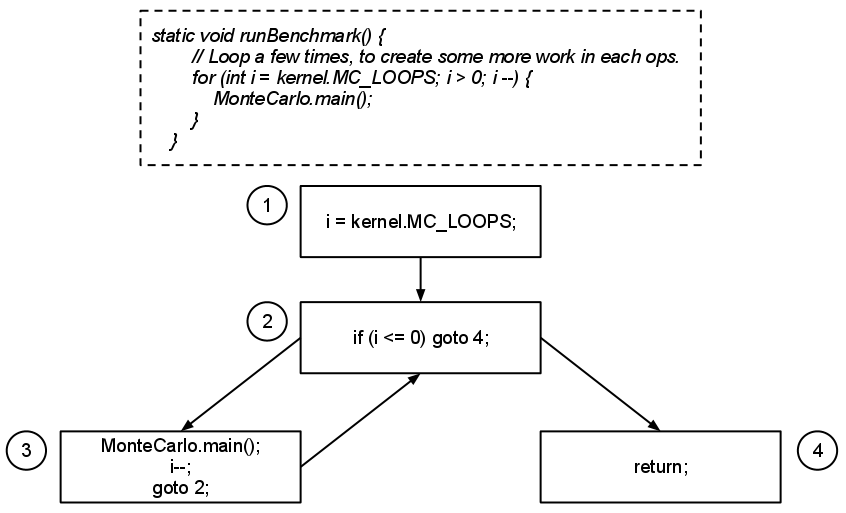
\includegraphics[width=8cm]{imgs/cfg.png}
\caption{An example of a control flow graph for a the \textit{rubBenchmark} method of \textit{SciMark} benchamrk from the \textit{SPECjvm2008} benchmarks
\cite{specjvm2008}.}
\label{fig:cfg}
\end{figure}

% \cite{baba2007design, ball1996efficient, duesterwald2000software, merten1999hardware}

\section{Motivation}
\label{sec:motivation}

\section{Related Work}
\label{sec:bg}

\section{Implementation}
\label{sec:implementation}

\subsection{Path Description Model}
\subsection{Path Enumeration}
assumptions: generate cfg for each method (useless to generate for a whole class, some classes do not have defined entry points), a path through the loop
represents all paths that take the loop once or more (to prevent unbounded number of paths).
generate cfg
feature extraction
\subsection{Dataset Generation}
specjvm2008
training set, test set
clustering training data to get estimates for hot, cold. show graph of 4 datasets
labeling both training and test data to get their ground truth
train bayes net with various training data and test the test data against it


\section{Experimental Results}
\label{sec:results}

\section{Discussion and Future Work}
\label{sec:difficulties}

\section{Conclusion}
\label{sec:conc}

% \begin{figure}[t!]
% \centering
% \includegraphics[width=6cm]{}
% \caption{Chan-Vese Curve Fitting}
% \label{fig:fitting}
% \end{figure}

% \begin{table*}[h!t!]
% \centering
% \begin{tabular}{ c | c |c}
% \textbf{Criteria} & \textbf{Goal} & \textbf{Applies to Model}\\
% \hline\hline
% Detecting Boundaries & Ability to correctly detect object boundaries of simple objects& Both Models\\
% \hline
% \end{tabular}
% \centering
% \caption{Evaluation Criteria}
% \label{tab:criteria}
% \end{table*}


{\small
\bibliographystyle{ieee}
\bibliography{references}
}
% insert where needed to balance the two columns on the last page with
% biographies
%\newpage

\end{document}